
\chapter{Fundamentos}

\section{Estado del Arte}\label{SOTA}

El Procesamiento del Lenguaje Natural, como cualquier tarea llevada a cabo por un algoritmo de Machine Learning, se basa en el análisis de un conjunto de rasgos del objeto a procesar, con la finalidad de realizar inferencias que permitan al sistema computarizado interactuar con el usuario.
\\
Para la tarea de  AP no es diferente, por lo que la mayoría de los trabajos se dirigen al desarrollo de una efectiva selección de rasgos, estableciéndose dos categorías fundamentales; los rasgos de estilo y los de contenido.  
\\
El análisis de estilo se enfoca en la detección de rasgos estilísticos del autor que sean lo suficientemente invariantes a lo largo de los pasajes escritos, pero que varíen de un autor a otro. Ejemplos de estos podrían ser la longitud media de las oraciones o la cantidad esperada de símbolos de puntuación, emoticones, preposiciones o  adverbios en un párrafo.
\\
Por otra parte el análisis de contenido se enfoca en la información contextual siguiendo la misma estrategia del análisis de estilo, i.e., llevar información estadística de la presencia de determinado conjunto de palabras o estructuras gramaticales. Este tipo de rasgos incluye el uso de n-gramas de palabras y caracteres, \textit{slang words}\footnote{ \textit{slang} se refiere a un lenguaje muy informal empleado por un grupo particular de personas.}, Bolsas de Palabras (\textit{Bag of Words} BoW) \citep{DBLP:conf/clef/Pizarro19,DBLP:conf/clef/Valencia-Valencia19}, palabras concluyentes (e.g., finalmente, para concluir, en conclusión, etc.)  y lexicones de palabras.
Dentro de este último método para categorizar palabras, el más empleado es el sistema \textit{Linguistic Inquiry and WordCount LIWC} \citep{pennebaker2015development} el cual contiene alrededor de 70 diccionarios de lexicones divididos en categorías como; Preocupaciones personales (\textit{Personal Concerns}), Discurso informal (\textit{Informal Speech}), Impulsos (\textit{Drives}) y necesidades fundamentales (\textit{Basics Needs}), etc.
\\\\
Estos dos grupos de rasgos, de estilo y contenido, son ortogonales puesto que los rasgos que se tienen en cuenta para capturar estilo, son precisamente aquellos que son independientes del tópico, por lo cual se ha hecho habitual el uso de enfoques que los combinen a ambos. Por otro lado el empleo de elementos contextuales implica introducir en el proceso de clasificación un sesgo hacia una clase que este más representada por determinado tema, e.g., según \citep{schler2006effects} estos rasgos pueden facilitar la determinación del sexo del autor ya que por ejemplo los hombres mayormente tienden a hablar de política y noticias, mientras que las mujeres se muestran más interesadas por la moda, fiestas y prendas de vestir; sin embargo es posible encontrar una mujer que regularmente postee tweets relacionados con deportes o automóviles, luego este perfil sería potencialmente mal clasificado por un modelo de AP basado en rasgos de contenido.
\\
La mayoría de los trabajos de Machine Learning han usado métodos de clasificación tradicionales como Regresión Logística (Logistic Regression LR) \citep{DBLP:conf/clef/Valencia-Valencia19}, Máquina de Vectores de Soporte (\textit{Support Vector Machines} SVM) \citep{DBLP:conf/clef/Pizarro19}  y Bosques Aleatorios (\textit{Random Forest} RF) \citep{DBLP:conf/clef/Johansson19} combinando conjuntos de rasgos que responden a estas clasificaciones.
\\
\\
 Con la introducción del Deep Learning en el NLP esta tendencia a la extracción manual de rasgos de tipo estadístico ha sido desplazada por el aprendizaje de rasgos abstractos que representan a las estructuras gramaticales atendiendo no solamente a su significado semántico como elementos aislados del texto, sino que tienen en cuenta además el contexto en el que son empleados, facilitando la comprensión y clasificación de los textos tanto a los propios modelos de DL como a los tradicionales de ML. Este tipo de enfoques se basan fundamentalmente en el uso de \textit{embeddings} preentrenados con distintas estrategias \citep{DBLP:conf/clef/JooH19,DBLP:conf/clef/Lopez-Santillan19}, principalmente Word2Vec \citep{DBLP:conf/nips/MikolovSCCD13}, Glove\citep{pennington2014glove} y Fasttext\citep{bojanowski2016enriching}.
 \\
 Las Redes Neuronales Artificiales como mecanismos de aprendizaje y clasificación, por su parte han logrado un desempeño superior a los métodos tradicionales de ML en muchas tareas de NLP, teniendo en cuenta que aprenden a decidir que elemento del texto tomar como rasgo significativo a la hora de modelar los objetos. Esquemas especializados en análisis de secuencias, como las Redes Neuronales Recurrentes (RNN) \citep{DBLP:conf/clef/DiasP19,bakhteev:2020} y las arquitecturas \textit{Transformers} (Transformadoras) \citep{iyer:2020,baruah:2020} se han empleado satisfactoriamente para el perfilado de autores en los últimos años, pero también se ha extendido el uso de arquitecturas diseñadas inicialmente para el tratamiento de otro tipo de información estructurada como las imágenes, tal es el caso de las Redes Neuronales Convolucionales (CNN) \citep{DBLP:conf/clef/PetrikC19,DBLP:conf/clef/Lopez-Santillan19}.
 \\
 \\
 En los últimos años dentro de PAN se han propuesto tareas de perfilado que van desde la predicción de sexo y variedad del idioma  hasta la detección de perfiles manejados por bots y perfiles que tienden a difundir discursos de odio en el medio social. En la mayoría de estas tareas los trabajos con un mejor desempeño se han enmarcado en técnicas tradicionales de ML, tal es el caso de \citep{basile:2017} en la tarea \textit{Gender and Language Variety Identification in Twitter at} PAN 2017, quienes emplearon rasgos construidos a partir de una medida no estándar de frecuencia de términos sobre unigrama de palabras y n-gramas de caracteres para entrenar una SVM y \citep{martinc:2017}  que combinaron n-gramas de palabras, caracteres y Elementos del Discurso (\textit{Part of Speech} POS), además de información de sentimientos relacionada con el uso de emojis y conteo de elongación de caracteres, con otros rasgos de estilo para modelar el perfil y entrenar un Regresor Logístico. 
 \\
 La tarea \textit{Bots and Gender Profiling in Twitter at} PAN 2019\footnote{\url{https://pan.webis.de/clef19/pan19-web/author-profiling.html}} consistente en determinar si una cuenta de Twitter pertenece a un bot o a un humano y en el segundo caso, inferir el sexo; \citep{DBLP:conf/clef/Pizarro19} obtuvo la mejor precisión con una SVM, combinando representaciones de los tweets mediante \textit{tf-idf} de n-gramas de palabras y caracteres. De igual forma \citep{DBLP:conf/clef/Johansson19} trató de dar solución a la tarea empleando ML con Random Forest y rasgos de estilo como logitud de los tweets, número de letras mayúsculas, URLs, menciones, cantidad de RTs, así como rasgos de contenido, específicamente ocurrencia de términos y etiquetas de POS.
 \\ 
 Nuevamente en PAN 2020 en la tarea \textit{Profiling Fake News Spreaders on Twitter}\footnote{\url{https://pan.webis.de/clef20/pan20-web/author-profiling.html}}, para detectar divulgadores de noticias falsas, \citep{pizarro:2020} se basó en la combinación de vectores de \textit{tf-idf} de n-gramas de palabras y caracteres para representar los tweets y clasificar los perfiles con una SVM. Mientras el modelo propuesto por \citep{buda:2020} consistió en un Regresor Logístico que combina las predicciones de cinco submodelos: (i) n-gramas con Regresor Logístico,(ii) n-gramas con SVM, (iii) n-gramas con Random Forest, (iv) n-gramas con XGBoost y (v) XGBoost con features de estilo.
 \\
Diversos modelos de DL empleando las arquitecturas citadas anteriormente (e.g., RNN y CNN) han sido propuestos a lo largo de estas competiciones, aunque ninguno de ellos mostró una precisión superior a la de los métodos tradicionales de ML. Sin embargo, en la tarea \textit{Profiling Hate Speech Spreaders on Twitter at} PAN 2021 \footnote{\url{https://pan.webis.de/clef21/pan21-web/author-profiling.html}}, consistente en determinar cuando un perfil era divulgador de contenido relacionado con el odio a grupos sociales específicos, el modelo con mejor desempeño, propuesto por \citep{sinno:2021} empleó una Red Neuronal Convolucional sobre la representación de los perfiles con \textit{embeddings} de palabras. 
\\\\
Uno de los mayores problemas con los enfoques predominantes es que los rasgos extraídos son muy dependientes del contexto lo cual puede crear una alta sensibilidad de los modelos ante datos que no correspondan a los corpus con los que han sido refinados sus parámetros o como ya hemos expuesto tengan un sesgo hacia alguna clase. Por ejemplo \citep{Newman2008GenderDI} expone que las mujeres tienden a usar emoticones con mayor regularidad que los hombres, lo contrario de lo concluido por \citep{Schwartz2013PersonalityGA}. Esto nos sugiere que métodos tan rigurosamente refinados como lo son los dependientes de rasgos manualmente extraídos tienen una menor robustez ante arquitecturas \textit{End-to-End} como las de Deep Learing.

\section{Marco Teórico}

En este epígrafe se realiza un acercamiento hacia los temas y arquitecturas de Machine Learning necesarios para la comprensión de los modelos propuestos en el trabajo.

\subsection{LSTM: Long Short-Term Memory Neural Networks}

	Las LSTM son un tipo de Redes Neuronales Recurrentes, las cuales están especializadas en el análisis de datos secuenciales. 
	Las RNNs tienen una unidad principal (la unidad recurrente) la cual explora la secuencia de datos de entrada de un elemento a la vez, ya sea de izquierda a derecha o viceversa. Al analizar un elemento para determinar su estado oculto, se comparte la información capturada en pasos anteriores del recorriendo. Esto es, sea $h_{t-1}$ el último estado oculto computado, $x_t \in \Re^d$ el $t-esimo$ elemento de la secuencia de entrada y $f$ una función de no linealidad. El estado oculto actual, se define como:
	\begin{equation}
		h_t = f(W_xx_t + W_hh_{t-1} + b_h)
		\label{rrn_form}
	\end{equation}
	Donde $W_x \in Re^{n_u\times d}$ y $W_h \in Re^{n_u\times n_u}$ son matrices de parámetros y $b_h \in R^{n_u}$ el término de sesgo (\textit{bias}), con $n_u$ el número de neuronas y $d$ la dimensión de los vectores que representan a los elementos de la secuencia.
	De esta forma la arquitectura aprende a considerar la información que tiene determinada influencia sobre el elemento de la secuencia que se analiza en cada paso como se muestra en la \figurename~\ref{rnn}, lo que le otorga una especie de ``memoria''.
	\begin{figure}[!thb]
		\begin{center}
			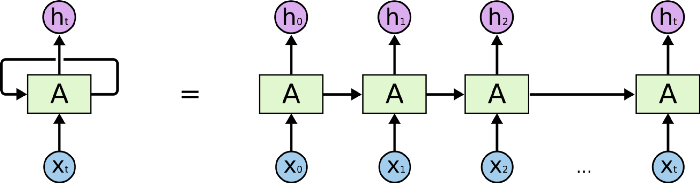
\includegraphics[width=250pt]{images/rnn.png}
		\end{center}
		\caption[Red Neuronal Recurrente]{Red Neuronal Recurrente sobre la secuencia $X_t$. \citep{agarwala2017music}}
		\label{rnn}
	\end{figure}
	\\
	Sin embargo, debido a que en las RNNs durante el proceso de \textit{backpropagation}, en el que se ajustan los parámetros de la red, cada neurona en la unidad principal calcula su gradiente para un paso del recorrido de la secuencia con respecto a su estado en el paso posterior, mediante la ley de la cadena, ocurre un decrecimiento exponencial de los valores de las derivadas parciales conocido como \textit{gradient vanishing}, lo que hace que los parámetros a penas se actualicen y se dificulte el aprendizaje de relaciones a largo plazo, de aquí su ``Short-Term Memory''.
	\\
	Esta limitación es lo que las LSTM tratan de solucionar introduciendo compuertas que deciden que información preservar u ``olvidar'' de los estados previos en el recorrido por la secuencia de la siguiente forma:
	\\
	Sean $W_f, W_i, W_o \in \Re^{n_u\times d}$ y $U_f, U_i, U_o \in \Re^{n_u\times n_u}$ las matrices de parámetros de la compuerta de ``olvidar '', entrada y salida respectivamente y $b_f, b_i, b_o \in \Re^{n_u}$ sus respectivos términos de bias:
	
	\begin{equation}
		\begin{split}
		i_{t} &= \sigma(W_i x_t + U_i  h_{t-1} + b_i)\\
		o_{t} &= \sigma(W_o x_t + U_o h_{t-1} + b_o)\\
		f_t &= \sigma(W_{f} x_t + U_f   h_{t-1} + b_f) 
		\end{split}
		\label{lstm_gates}
	\end{equation}
	\\
	Una codificación potencial $\hat{c}_t$ considerando el elemento $x_t$ de la secuencia y el estado previo $h_{t-1}$ esta dado por:
	\begin{equation}
		\hat{c}_{t} = \sigma(W_cx_t + U_c h_{t-1} + b_c)
		\label{lstm_pu}
	\end{equation}
	\\
	Donde $W_c\in\Re^{n_u\times d}$, $U_c\in\Re^{n_u\times n_u}$ y  $b_c\in\Re^{n_u}$. Luego la codificación $x_t$ teniendo en cuenta la codificación del elemento anterior y $h_t$ quedan definidos por:
	 \begin{equation}
	 	\begin{split}
	 		c_{t} &= f_tc_{t-1} +i_t\tanh(\hat{c}_{t})\\
	 		h_t &= o_t\tanh(c_t)
	 	\end{split}
	 	\label{lstm_hstate}
	 \end{equation}
 
 
\subsection{Redes Neuronales Convolucionales sobre secuencias}
	
	La arquitectura de una CNN \citep{lecun1998gradient} sobre una secuencia de texto es capaz de capturar dependencias temporales a corto plazo mediante filtros unidimensional que analizan n-gramas de palabras o caracteres y cuyos parámetros son compartidos durante cada paso de manera similar a las LSTM.
	\\
	Esto es, sea $X \in \Re^{l\times d}$ la secuencia de entrada de longitud $l$ donde cada elemento es un vector $d-dimensional$, $F_k$ el conjunto de filtros con ventana $k$ de una capa convolucional, cada uno de los ${F_k}_i \in \Re^{k\times d}$ son inicializados de manera independiente y de la misma forma aprenden a capturar relaciones a corto plazo  dentro en $X$. La operación convolución (\textit{conv-op}) transforma a $X$ en una nueva secuencia $X' \in \Re^{(l - k) \times n_f}$ donde $n_f = |F_k|$ de la siguiente forma:
	
	\begin{equation}
		X'_{ij} = \sum X_{[i:i+k]} * {F_k}_j ~~~ para ~~~ j \in [0, F_k-1], \;i \in [0, l-k]
	\end{equation}
	\\
	Como se puede observar en la \figurename~\ref{cnn} donde se representa un paso del desplazamiento de la ventana del filtro:
	\begin{figure}[!thb]
		\begin{center}
			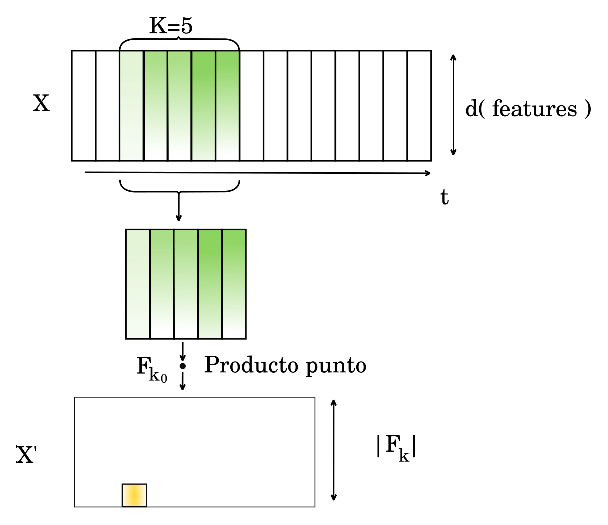
\includegraphics[width=250pt]{images/cnn.eps}
		\end{center}
		\caption[Operación Convolución. CNN]{Operación convolución sobre $X$ con filtros de tamaño de ventana k. }
		\label{cnn}
	\end{figure}
	\\
	Vinculada a la \textit{conv-op} en este tipo de arquitectura se suele emplear además una capa de \textit{pooling}, en la cual se combinan los valores de elementos en una vecindad para reducir la dimensionalidad de la secuencia seleccionando los valores más importantes de dicha vecindad, esta operación de \textit{pooling} con una ventana de tamaño $k$  sobre una secuencia $X$ esta definida por:
	\begin{equation}
		X'_i = f(X_{[i:i+k]}) ~~ para ~~~  \;i \in [0, l-k]
	\end{equation}
	\\
	Donde $f$ es la función de \textit{pooling}, regularmente empleadas las funciones $Max$ o $Avg$.
		
\subsection{Mecanismos de Atención}\label{atencion}

	Los mecanismos de atención, son técnicas de procesamiento de las entradas de una arquitectura o de algún resultado intermedio que permiten a la red prestar mas ``atención'' a elementos específicos de una secuencia o establecer la importancia relativa sobre un elemento del resto. En la práctica, la atención permite a las redes neuronales aproximarse al mecanismo de atención visual que utilizan los humanos.

	\subsubsection{Self-Attention}
	
		Sea $x_t$ la representación del $t-esimo$ elemento de la secuencia, una capa de \textit{self-attention} (auto-atención), captura en una matriz $A$ cuan similar es $x_t$ con sus vecinos. Específicamente $\alpha_{t, t'} \in A$ expresa la relación de $x_t$ con $x_t'$ y de manera similar al de una red recurrente este valor se calcula como:
		\begin{equation}
			\begin{split}
				g_{t, t'} &= \tanh(W_{x}x_t + W_{x{t'}}x_{t'} + b_g)\\
				a_{t, t'} &= \sigma({W_{a}g_{t, t'} + b_{a}}) 
			\end{split}
		\end{equation}
		\\
		Donde $\sigma$ es la función sigmoide, $W_{x}, W_{x{t'}} \in \Re^{n_u \times d} $ son las matrices de parámetros encargadas de codificar la información de $x \text{ y } x'$ para expresar su compatibilidad, $W_a \in \Re^{n_u \times n_u}$ la matriz de parámetros correspondiente a su combinación no lineal y $b_g \text{ y } b_a$ los correspondientes términos de bias.
		\\
		A partir de $A$ el estado correspondiente al vector $x_t$, $\hat{x}_t$ está dado por la suma ponderada de sus elementos vecinos $x'_t$:
		
		\begin{equation} \label{attention}
			\hat{x}_t = \sum \limits_{i=0} a_{t,t'}x_{t'}
		\end{equation}
		\\
		Luego $\hat{x}_t$ expresa cuan atendido debe ser $x_t$ condicionado por el contexto de su vecindad.
	
	\subsubsection{Scaled Dot-Product Attention}
		
		El mecanismo \textit{Scaled Dot-Product Attention} (Atención con Producto-Punto Escalado) primero se mapea cada elemento de la secuencia con tres representaciones (\textit{query} y un par \textit{key-value}) para calcular el índice de compatibilidad entre cada par de elementos. Luego, para cada $x_t$ es evaluada su compatibilidad con respecto a cada uno de los  elementos vecinos relacionando su \textit{query} ($q_t$) con las \textit{keys} de los vecinos ($k_{t'}$), estos valores de compatibilidad son escalados y normalizados con la función $softmax$ y empleados para ponderar los vectores de \textit{value} ($v_t$). Finalmente la representación de $\hat{x}_t$ es calculada como la suma ponderada de los $v_t$. En forma matricial queda expresado como:
		
		\begin{equation}
			Attention(Q, V, K) = softmax(\frac{Q\times K^T}{\sqrt{d_k}})\times V
			\label{dotP-att}
		\end{equation} \\
		Donde $Q, K \in \Re^{n\times d_k} \text{ y } V \in \Re^{n\times d_v} $ son el resultado del producto de las matrices de parámetros de \textit{query}, \textit{key} y \textit{value} con los elementos de la secuencia respectivamente, por tanto en la fila $t$ contienen el mapeo del elemento $x_t$ y  $d_k,d_v$ corresponden a la dimensionalidad de las vectores de \textit{key} y \textit{value} respectivamente.
		
\subsection{Transformers}

	La arquitectura Transformer (\figurename~\ref{transformer}) basada en mecanismos de atención, específicamente \textit{multihead attention} \citep{vaswani2017attention}, está diseñada para tratar problemas de \textit{machine translation} y la conforman dos módulos, el primero conocido como \textit{Encoder} (Codificador) es alimentado con una secuencia textual y se encarga de encontrar una codificación para cada elemento teniendo en cuenta la información de su contexto. El segundo módulo, \textit{Decoder} produce los elementos de una nueva secuencia en el modelado de lenguaje, haciéndolo de uno a la vez y teniendo en cuenta los elementos generados anteriormente y las codificaciones obtenidas por el Encoder de la secuencia de entrada.
	\\
	La principal ventaja de las Transformers con respecto a las arquitecturas secuenciales más tradicionales, e.g., GRU y LSTM es que en vez de analizar la información textual en una dirección, esta toma en consideración la entrada completa relacionando cada elemento con el contexto de su vecindad simultáneamente lo cual evita el problema de ``memoria'' a corto plazo de las RNN.  Sin embargo pudiera parecer que existe una pérdida de la percepción del tiempo al analizarlo todo a la vez, es por esto que ademas de representar el texto con un \textit{embedding} de palabras, se tiene en cuenta un \textit{encoding} de posición. 
	\begin{figure}[!thb]
		\begin{center}
			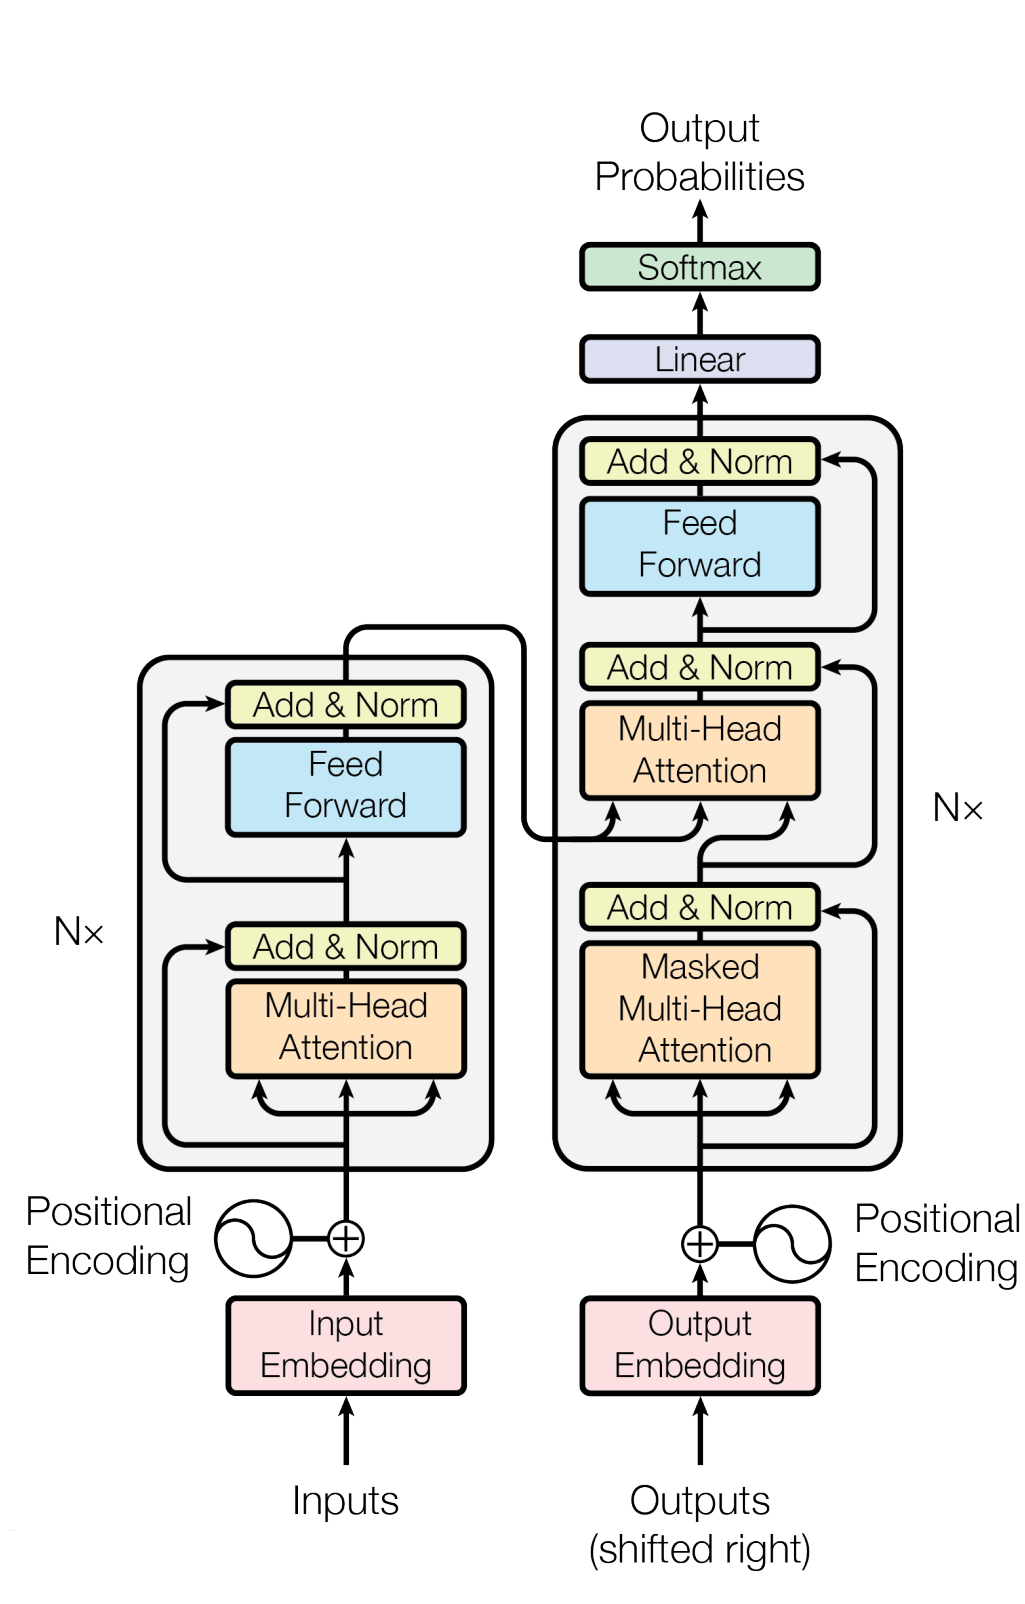
\includegraphics[width=.5\linewidth, height=.5\textheight]{images/transformer.png}
		\end{center}
		\caption[Arquitectura Transformer]{Arquitectura Transformer. Módulo Izquierdo, Codificador. Módulo Derecho, Decodificador. \citep{vaswani2017attention} }
		\label{transformer}
	\end{figure}
	\\
	En la \figurename~\ref{transformer} se observan cada uno de los módulos los cuales se apilan ($N_x$), i.e., antes de que el Decoder reciba la informacion codificada de la secuencia de entrada, esta transita por una serie de bloques codificadores haciendo uso de una red residual para prevenir cualquier pérdida de la información.
	\\
	Dentro de la mayoría de las tareas de NLP este tipo de modelo ha alcanzado nuevos estados del arte simplemente haciendo \textit{transfer learning} del modulo de Encoder hacia la tarea específica. Este módulo es entrenado en dos tareas: (i) predecir palabras enmascaradas de la secuencia; (ii) dadas dos oraciones, predecir si una está a continuación de la otra en el texto, lo cual hace que el modelo llegue a ``entender'' el funcionamiento del lenguaje y sea relativamente fácil de entrenar sobre otras tareas como el análisis de sentimientos. Para esta última tarea, dado el par de oraciones como una secuencia, se añade un \textit{token} [CLS] al inicio del cual su estado oculto se toma para realizar la clasificación y otro [SEP] al final de cada oración. 
	
\subsection{Redes Neuronales Convolucionales en Grafos}
	
	La principal diferencia entre las CNNs y las Redes Neuronales Convolucionales en Grafos (\textit{Graph Convolutional Neural Nets }GNN) es que las primeras están diseñadas especialmente para tratar datos regularmente estructurados (Euclideanos), mientras que las GNN son su versión generalizada capaz de extraer información en datos donde no existe una relación de orden entre un nodo y otro y las conexiones entre cada uno de ellos es variable (datos irregulares o datos estructurados no Euclideanos), estas dos propiedades son totalmente opuestas a las relaciones que existen entre los píxeles de una imagen (\figurename~\ref{euclidian-non}).
	\begin{figure}[!thb]
		\centering
		\subfigure[Datos Estructurados Euclideanos]{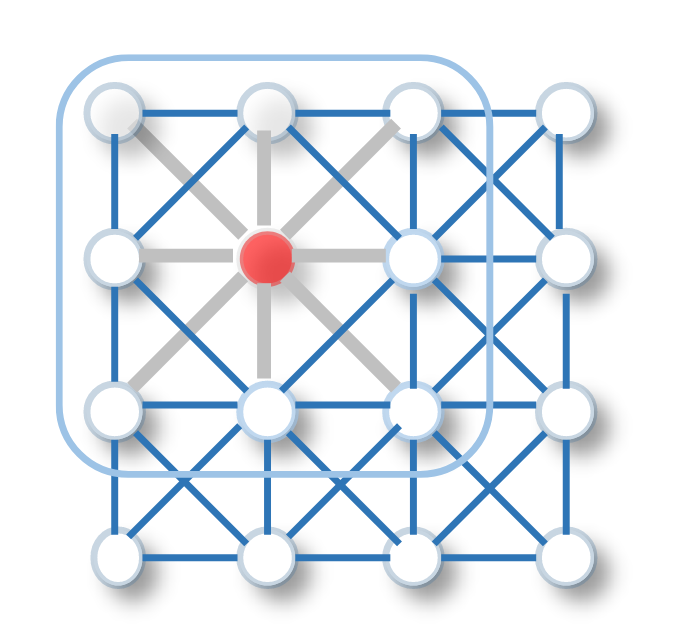
\includegraphics[width=0.35\textwidth]{images/cnn-gnn.png}} \hspace{10mm}
		\subfigure[Datos con Estructura No Euclideana]{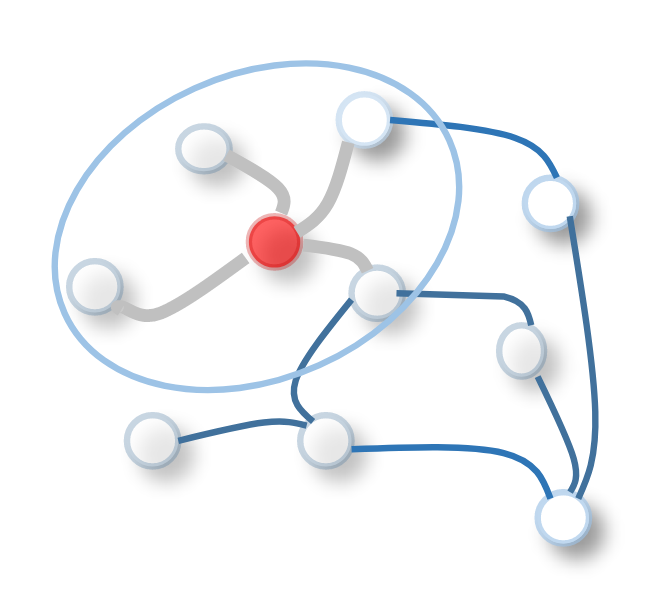
\includegraphics[width=0.35\textwidth]{images/gnn-gnn.png}} 
		\caption[Relación de Estructura en los Datos]{Relación de Estructura en los Datos. \citep{Wu_2021}}
		\label{euclidian-non}
	\end{figure}
	\\
	Un uso típico de las GNN es la clasificación de nodos en una estructura. En este tipo de problema el nodo $v$ se caracteriza por un conjunto de features $x_v$ y corresponde a una clase $t_v$. Dado un grafo $G = (V, E)$ parcialmente etiquetado, nuestro objetivo es predecir a que clase corresponde cada nodo no etiquetado. Mediante una GNN, cada nodo comparte información con su vecindad y transforma su representación a un estado $h_v$ de manera que exprese como este pertenece a su contexto. Específicamente,	
	\begin{equation}
		h_v = f(x_v, E_v, H_v, X_v)
	\end{equation}
	\\
	Donde $E_v = \{(i, j)| (i, j) \in E, v \in \{i, j\}\}$,  $H_v = \{h_u| u \in \mathcal{N}(v)\}$ con $\mathcal{N}(v)$ el conjunto de nodos de la vecindad de v y $X_v = \{x_u| u \in \mathcal{N}(v)\}$. Dentro del espacio imagen de $f$ es de nuestro interés que cada nodo tenga un estado $h_v$ unívoco, por lo que apoyándose en el teorema del punto fijo \citep{brown1988fixed} es posible encontrar en un proceso iterativo de actualizaciones con determinados parámetros para nuestra función $f$ este $h_v$ contextualizado. El proceso de actualizaciones llevado a cabo dado $f$ es conocido como paso de mensajes. Luego, en forma matricial el estado de todos los nodos en la actualización $t+1$ esta dado por:
	
	\begin{equation}
		H^{t+1} = F(H^t, X)
	\end{equation} 
	\\
	Con $H$ y $X$ matrices donde a cada fila $i$ le corresponde $h_i \text{ y } x_i$ respectivamente. Luego, la clasificación de un nodo es llevada a cabo mediante la una nueva función $g$:	
	
	\begin{equation}
		t_v = g(h_v, x_v)
	\end{equation}
	\\
	Muchos diseños de la función de agregación han sido estudiados \citep{kipf2017semisupervised} teniendo en cuenta propiedades de la topología del grafo y la simetría que debe cumplir el análisis de $\mathcal{N}$ i.e., $F$ no puede ser sensible al orden de agregación de la información. En este trabajo, hacemos uso específicamente de las GNN de tipo espectral \citep{Wu_2021} y la clasificación de G. Este tipo de enfoque no difiere mucho de la clasificación de nodos, pues sigue siendo fundamental la determinación de un estado para cada nodo que exprese su información contextual. Esta información contextual es agregada mediante una operación de \textit{pooling} para alimentar una red densa y proceder con la clasificación de la estructura.
	
%\subsection{Information Gain}
%
%	El índice de \textit{Information Gain }IG (Captura de Información) \citep{10.5555/3091696.3091731,sebastiani2002machine} mide cuanta información aporta un rasgo sobre una clase tomando en cuenta tanto la presencia como la ausencia del término en los documentos pertenecientes a la misma. El IG de un término $t$ en una clase $C$ está definido por:
%	
%	\begin{equation}
%		IG(t, C) = \sum_{c \in \{C, \bar{C}\}} \sum_{x \in \{t, \bar{t}\}} P(x, c) \log_2\frac{P(x, c)}{P(x)P(c)}
%	\end{equation}
%	\\
%	Donde las probabilidades están interpretadas en un espacio de eventos sobre los documentos, e.g., $P(\bar{t}, C)$ indica la probabilidad de que para un documento aleatorio $d$, el término $t$ no ocurra en $d$ y $d$ pertenezca a la categoría $C$. 